\section{Gleichstromnetzwerke}

\subsection{Pfeilsysteme}
\begin{multicols}{3}
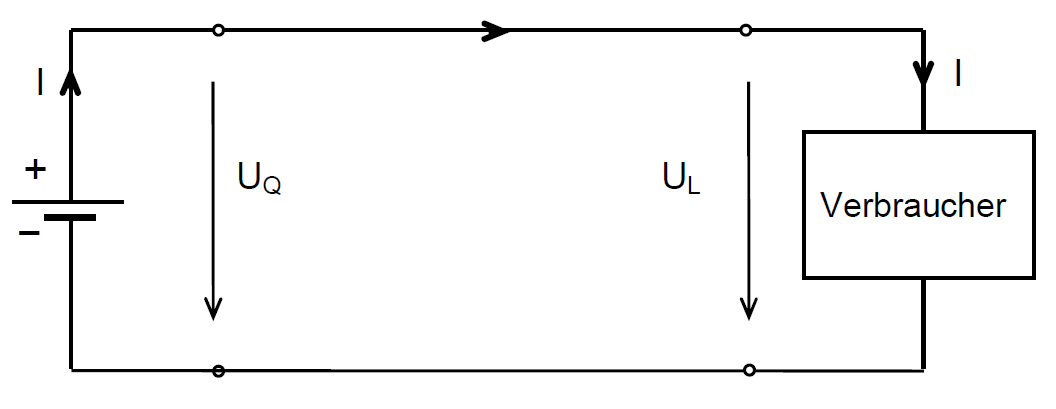
\includegraphics[width=0.35\textwidth]{pics/dcnet/pfeilsysteme}\\
\begin{itemize}
	\item Erzeuger-Pfeilsystem: Spannungs- und Strompfeil \textbf{entgegengesetzt}
	\item Verbraucher-Pfeilsystem: \textbf{gleiche} Bezugsrichtung f"ur Strom und Spannung
\end{itemize}
\end{multicols}
\begin{multicols}{2}
\subsection{lineare Widerst"ande}
$$U=R \cdot I \rightarrow G = \frac{1}{R}$$ \\

\subsection{Leistung an linearen Widerst"ande}
$$P=U \cdot I \ \rightarrow P=R \cdot I^2 = \frac{U^2}{R}$$

\subsection{Nonlineare Widerst"ande}
Als differenzielle Widerst"ande bezeichnet man die Steigung der Tangente an einem bestimmten Punkt.\\
$$r = \frac{\Delta U}{\Delta I} \rightarrow g = \frac{\Delta I}{\Delta U}$$\\

\subsection{Spezifischer Widerstand und Leitf"ahigkeit}
$$R=\frac{\rho \cdot \mathit{l}}{A}=\frac{\mathit{l}}{\sigma \cdot A} \qquad \lbrack \rho \rbrack = \frac{ \Omega \cdot mm^2}{m},\lbrack \sigma \rbrack = \frac{1}{\rho}, \lbrack \mathit{l} \rbrack = m$$

\subsection{Temperaturabh"anigkeit von Widerst"anden}
\begin{itemize}
	\item PTC: Kaltleiter, temp. hoch $\rightarrow$ Widerstand gross
	\item NTC: Warmleiter, temp. hoch $\rightarrow$ Widerstand klein
\end{itemize}
$$\Delta R = R_{20} \cdot \alpha_{20} \cdot \Delta \vartheta$$ $$\rightarrow R = R_{20} \cdot (1 + \alpha_{20} \cdot \Delta \vartheta)$$\\
$\alpha$ = Temperaturkoeffizient, $\alpha_{20}=\frac{\Delta R}{ R_{20} \cdot \Delta \vartheta} \rightarrow \lbrack \frac{1}{K} \rbrack$\\
0°C = 273,15K

\end{multicols}

\subsection{Ideale Spannungsquellen}
\begin{multicols}{4}
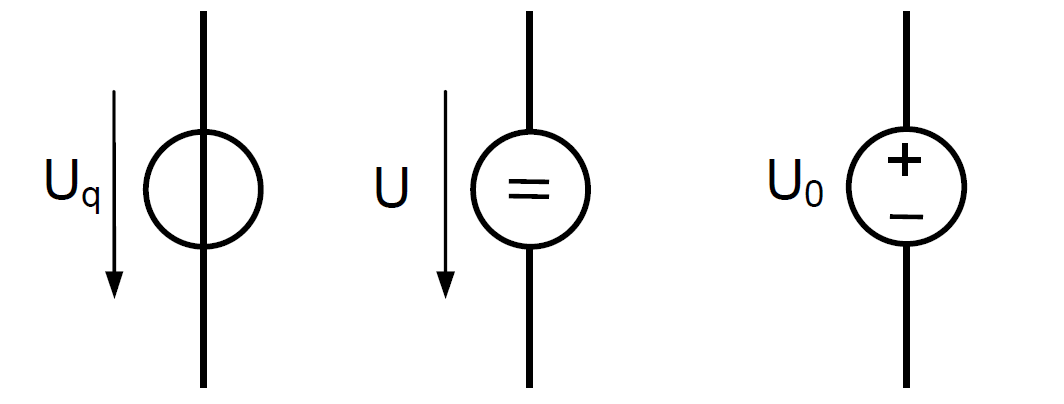
\includegraphics[width=0.20\textwidth]{pics/quellen/UQsymbole}\\
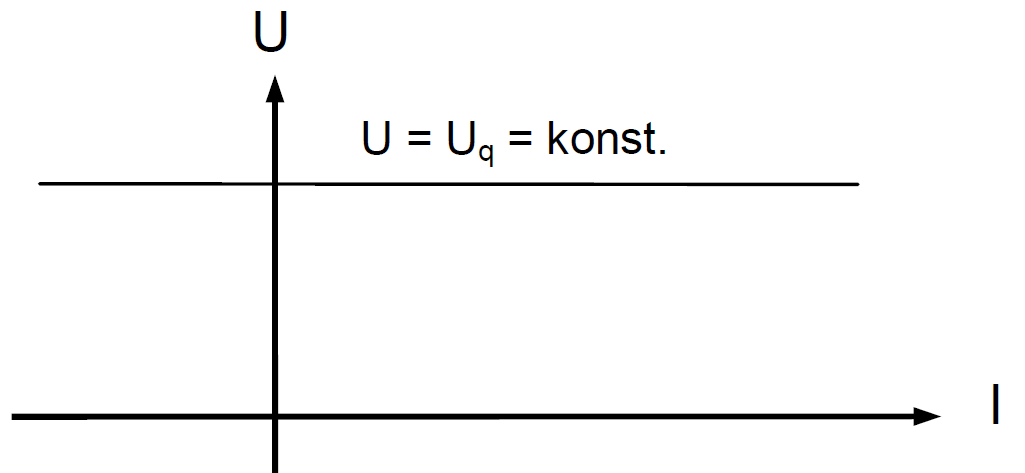
\includegraphics[width=0.20\textwidth]{pics/quellen/QUkennlinie}\\
Bei Quellenüberlagerung wird Spannungsquelle als Kurschluss betrachtet\\
\end{multicols}

\subsection{Lineare Spannungsquellen}
\begin{multicols}{4}
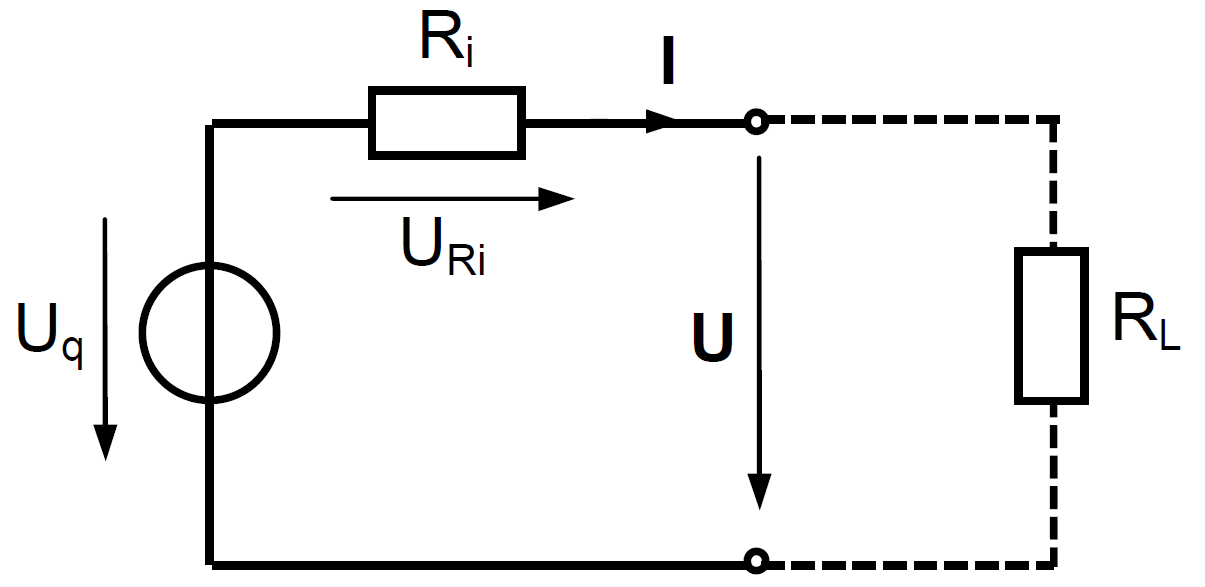
\includegraphics[width=0.20\textwidth]{pics/quellen/lUEquelle}\\
$U_q\ =$ Leerlaufspannung\\
$U\ =$ Klemmenspannung
$R_I\ =$Innenwiderstand
$R_I=\frac{U_q}{I_K}$\\
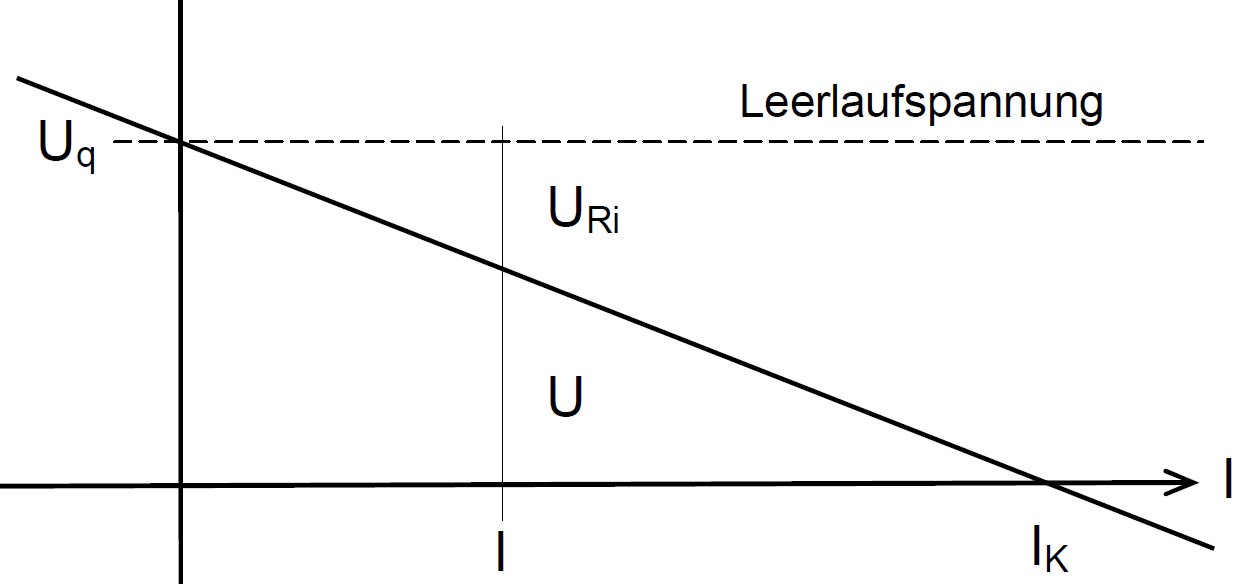
\includegraphics[width=0.20\textwidth]{pics/quellen/UIkennlinie}\\
$I_K\ =$Kurzschlussstrom $(U=0)$\\
\end{multicols}

\subsection{Ideale Stromquellen}
\begin{multicols}{4}
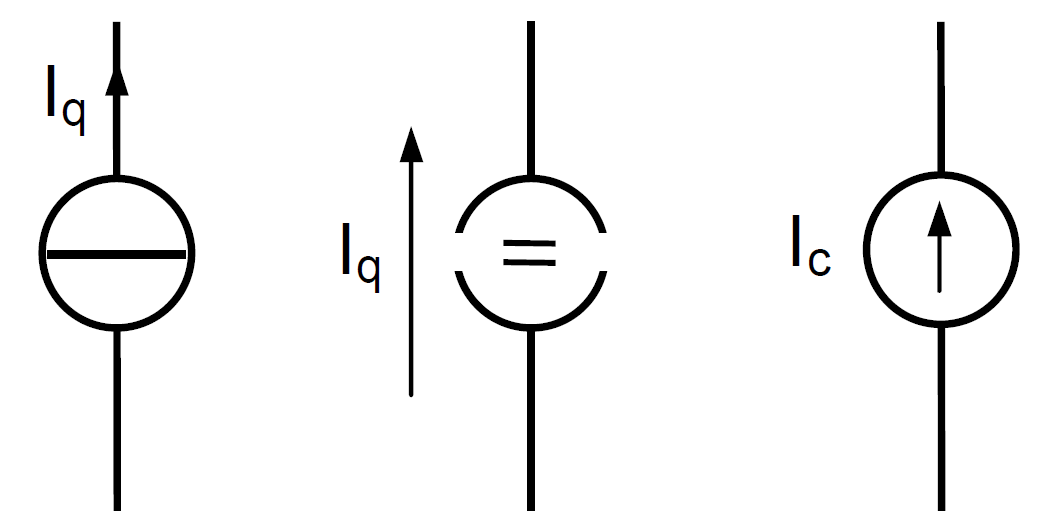
\includegraphics[width=0.20\textwidth]{pics/quellen/IQsymbole}\\
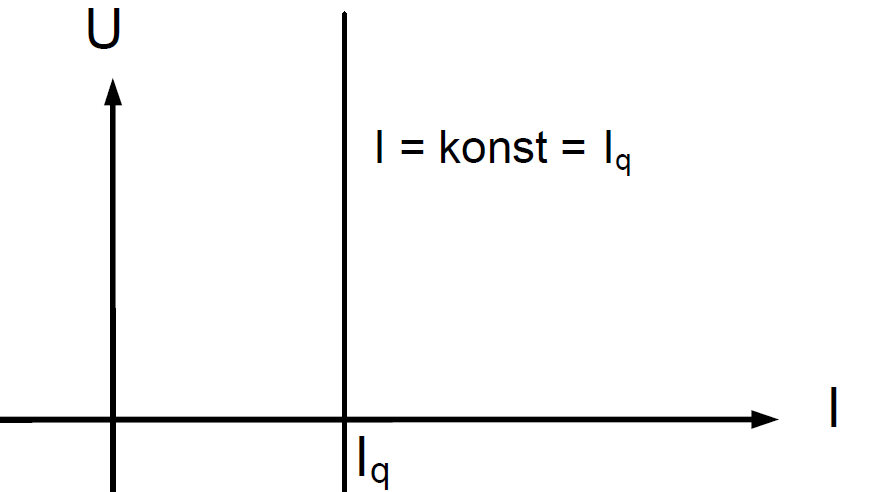
\includegraphics[width=0.20\textwidth]{pics/quellen/QIkennlinie}\\
Bei Quellenüberlagerung wird Stromquelle als Unterbruch betrachtet\\
\end{multicols}

\subsection{Lineare Stromquelle}
\begin{multicols}{4}
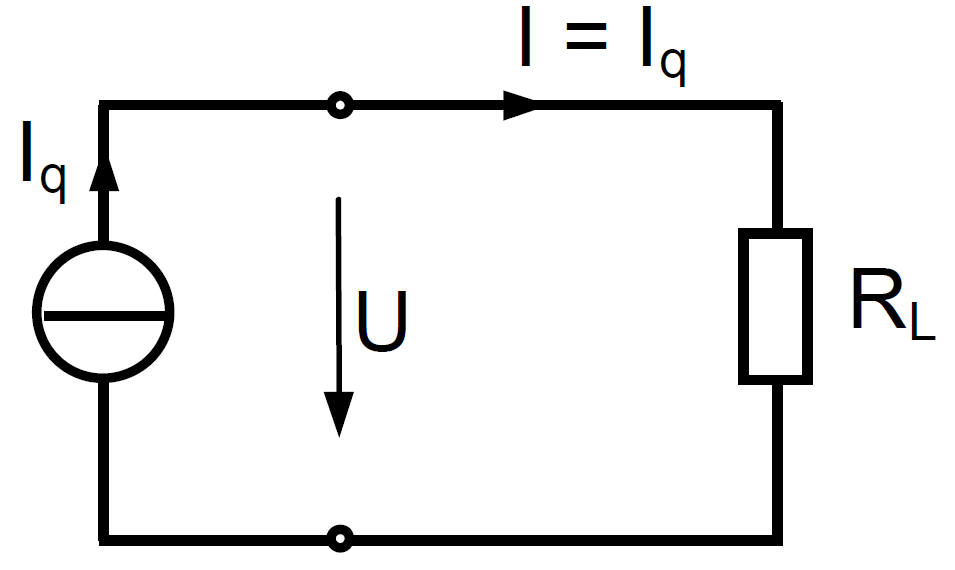
\includegraphics[width=0.25\textwidth]{pics/quellen/lIEquellen}\\
$R_i=\frac{U_0}{I_q}=\frac{U_0}{I_K}$\\
$\rightarrow{I_q} = {I_K}$\\
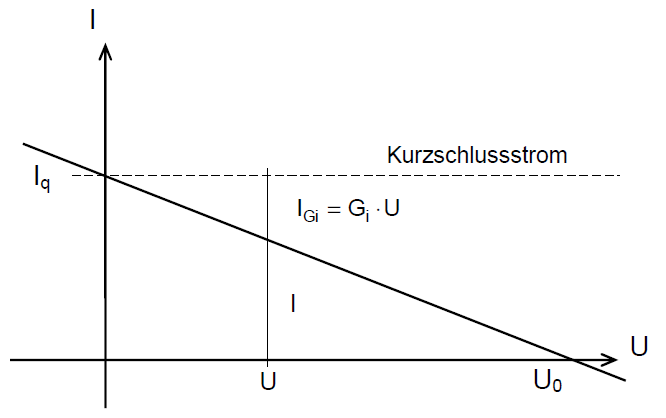
\includegraphics[width=0.20\textwidth]{pics/quellen/IUkennlinie}\\
$U_0=$Leerlaufspannung ($I=0!$)\\
\end{multicols}

\subsection{Ersatzschaltbild}
\begin{multicols}{3}
Nach Thévenin $\rightarrow R_i$ klein\\
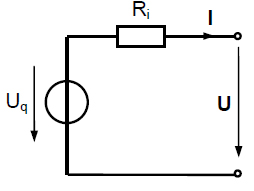
\includegraphics[width=0.2\textwidth]{pics/dcnet/ersatz_spannung}\\
Nach Norton $\rightarrow R_i$ gross\\
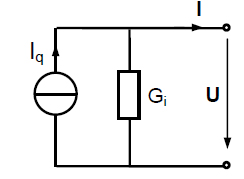
\includegraphics[width=0.2\textwidth]{pics/dcnet/ersatz_strom}\\
Formeln\\
$$ U_q = U_0  \rightarrow I_q = I_K $$\\
$$ R_i = \frac{U_q}{I_q} = \frac{U_0}{I_K} \rightarrow G_i = \frac{I_K}{U_0}$$\\
Umwandlung: $R_i$ ist bei beiden gleich!
\end{multicols}

\subsection{Lineare Quellen - nonlinearer Widerstand}
\begin{multicols}{2}
\begin{itemize}
\item Gegeben: - $U_q$, $R_i$ von linearer Quelle\\
 \hspace{1.6cm}- Kennlinie von nichtlinearem Widerstand\\
\item Gesucht: Klemenspannung $U_A$ und Strom $(I_A)$
\item Vorgehen: I-U-Kennlinie von beiden Zweipolen in Diagramm eintragen und Werte bei Arbeitspunkt ablesen:
\end{itemize}
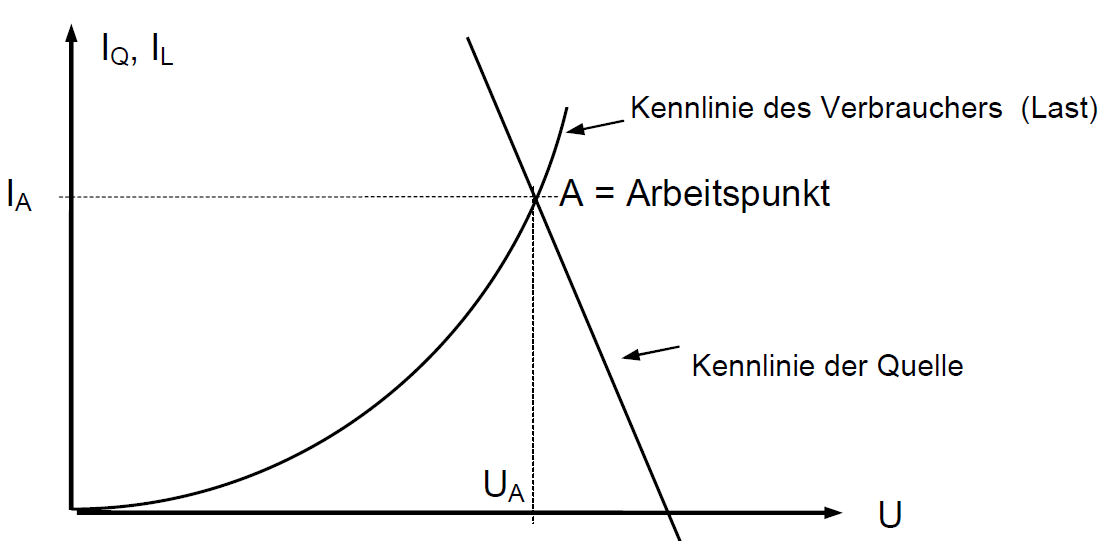
\includegraphics[width=0.3\textwidth]{pics/quellen/nonlineUI}
\end{multicols}

\subsection{Addition von nichtlinearen Zweipolen}
\begin{multicols}{2}
\subsubsection{Serieschaltung}
Teilspannungen bei gleichen Str"omen addieren.\\
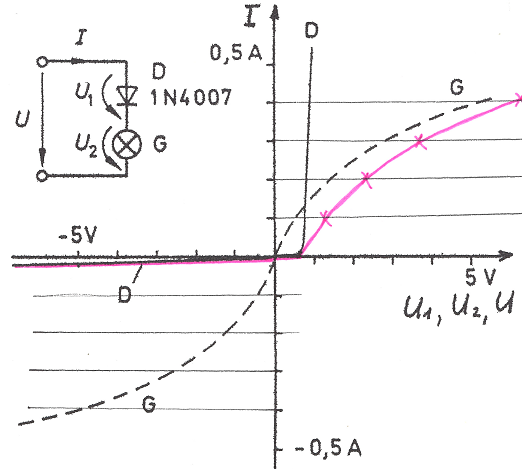
\includegraphics[width=0.3\textwidth]{pics/kennlinien/nonlinAddPar}
\subsubsection{Parallelschaltung}
 Teilstr"ome bei gleicher Spannung addieren.\\
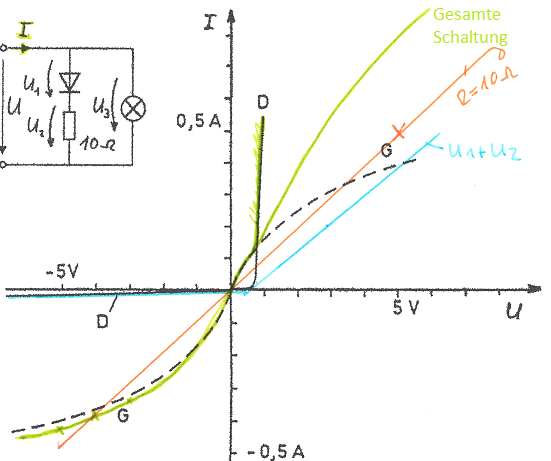
\includegraphics[width=0.32\textwidth]{pics/kennlinien/nonlinAddSer}\\
\end{multicols}

\subsection{Wirkungsgrad}
\begin{tabular}{ll}
Wirkungsgrad & $\eta = \frac{P_{ab}}{P_{zu}}$ \\[3pt]
& $ P_{zu} = P_{ab}+P_{verlust} $\\
& $ \eta_{tot} = \eta_1 \cdot \eta_2 \cdot \eta_3 $\\
Bei realen Quellen & $\eta = \frac{abgegebene Leistung}{abgeg. Leistung + innere Verlustleistung}$\\
Bei lin. U-Quelle & Innere Verluste bei Leerlauf = 0\\
& Bei Kurzschluss Max-Wert $P_{max} = R_i \cdot I_k^2$\\
Bei lin. I-Quelle & Innere Verluste bei Kurzschluss = 0\\
& Bei Leerlauf Max-Wert $P_{max} = G_i \cdot U_0^2$\\
\end{tabular}\\
\textbf{Vorsicht:} Obwohl die Schaltungen äquivalent sind, sind die inneren Verluste NICHT gleich!

\subsection{Leistungsanpassung}
Bei $R_i = R_L$ \\[3pt]
$P_{max} = \frac{U_q^2}{4 \cdot R_i} = \frac{I_q^2}{4 \cdot G_i}\rightarrow$ verfügbare Leistung am $R_L$\\[3pt]
$\eta$ beträgt 50\% $\rightarrow$ am $R_i$ wird gleich grosse Leistung umgesetzt wie am $R_L$\\

\subsection{Wheatstone Brücken}
%\subsubsection{Anwendung}
%\begin{itemize}
%\item Messungen von Widerständen (bei Wechselstrom: auch Bestimmung von L, C samt Verlustfaktor)
%\item In Verbindung mit Sensoren (Temp.- oder Druckabhängige Widerstände: Bestimmung von Temp, Kraft, etc.)
%\end{itemize}
\subsubsection{Speisung mit U-Quellen}
\begin{tabular}{lll}
Abgeglichene & Nicht abgeglichene & Mit $R_L$ belastet \\
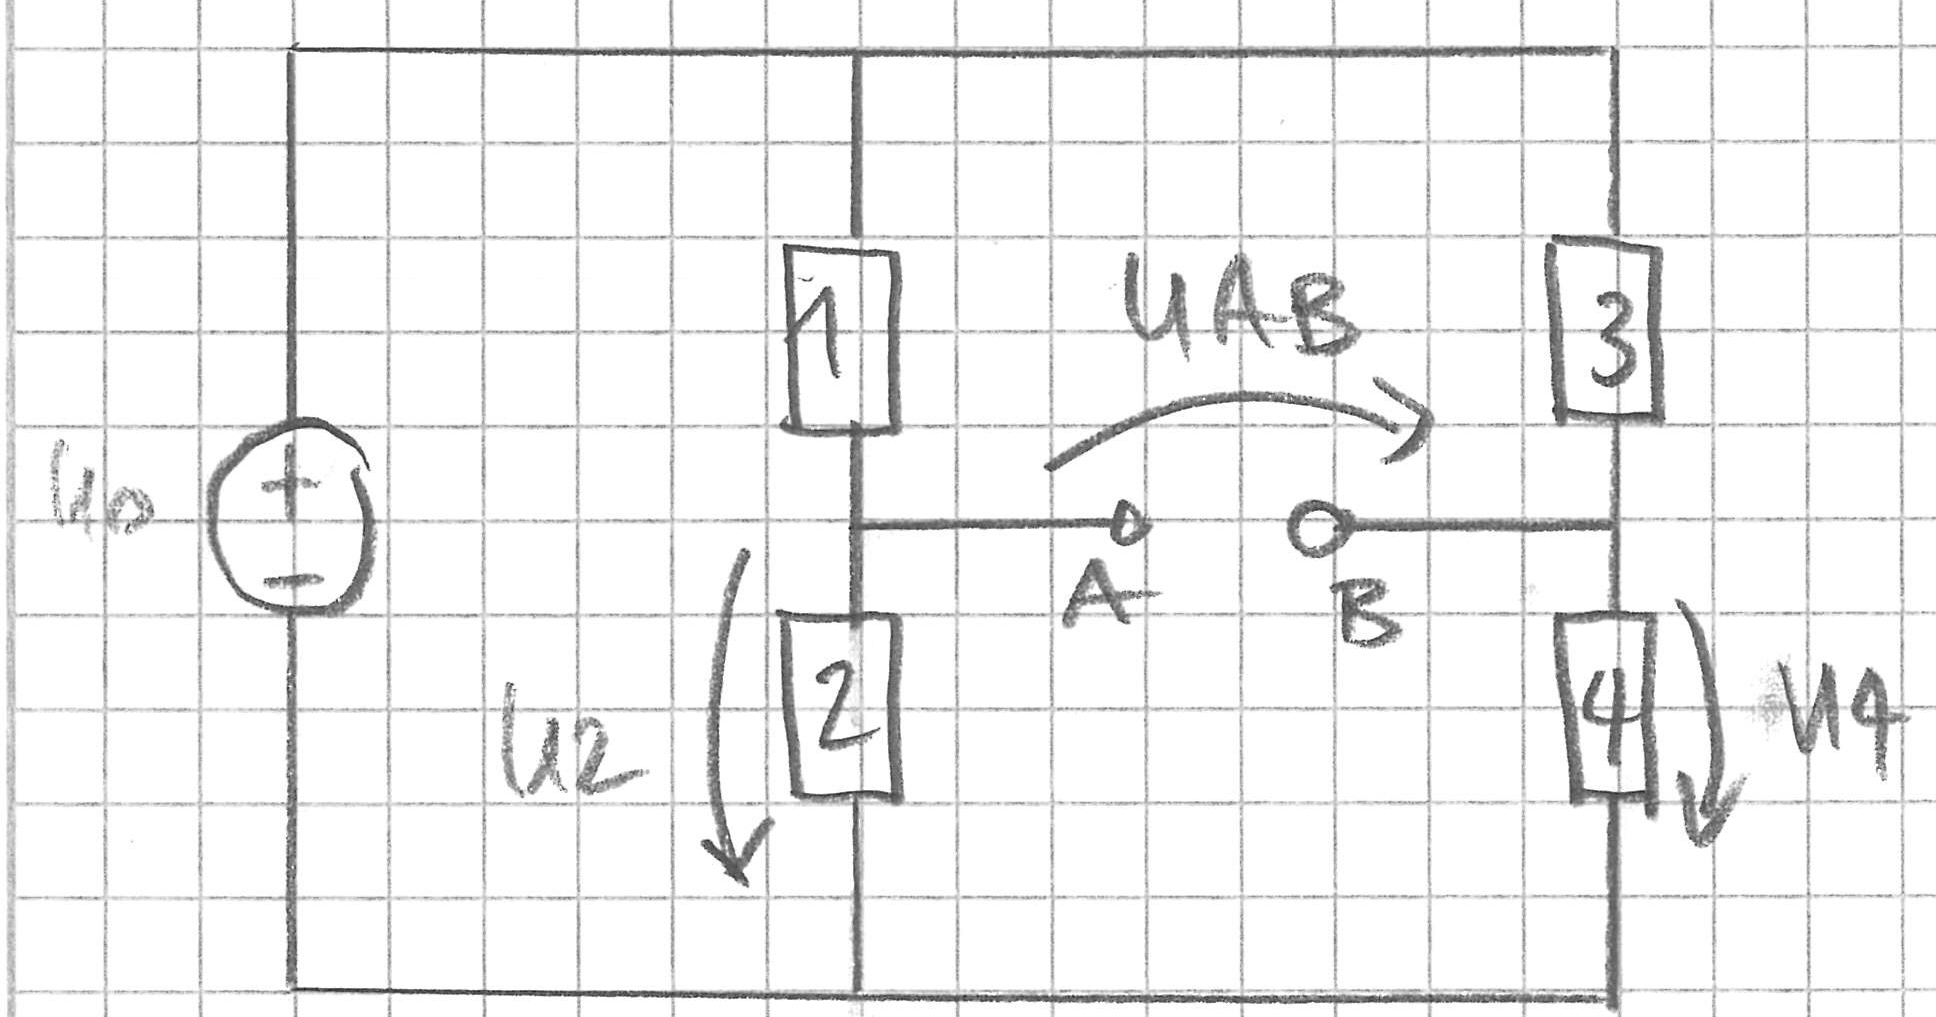
\includegraphics[width=0.3\textwidth]{pics/wheatstone/u_quelle_abgeglichen} & 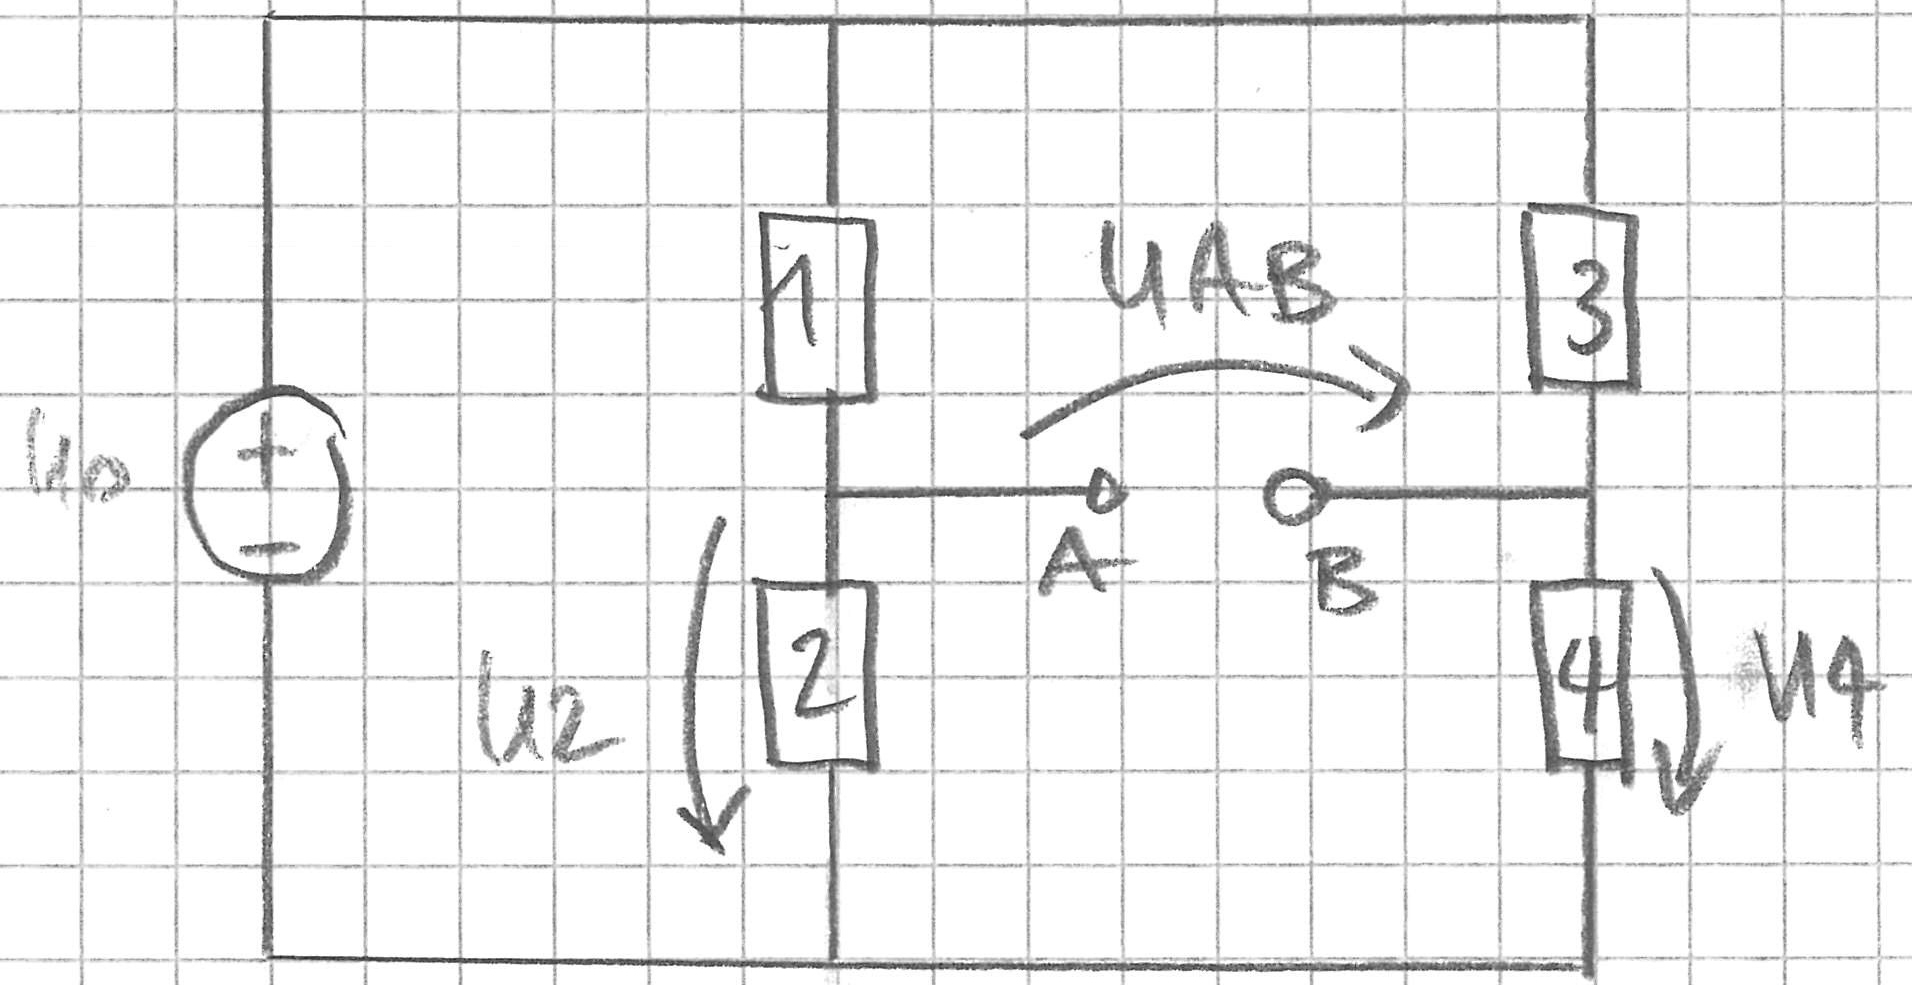
\includegraphics[width=0.3\textwidth]{pics/wheatstone/u_quelle_nicht_abgeglichen} & 
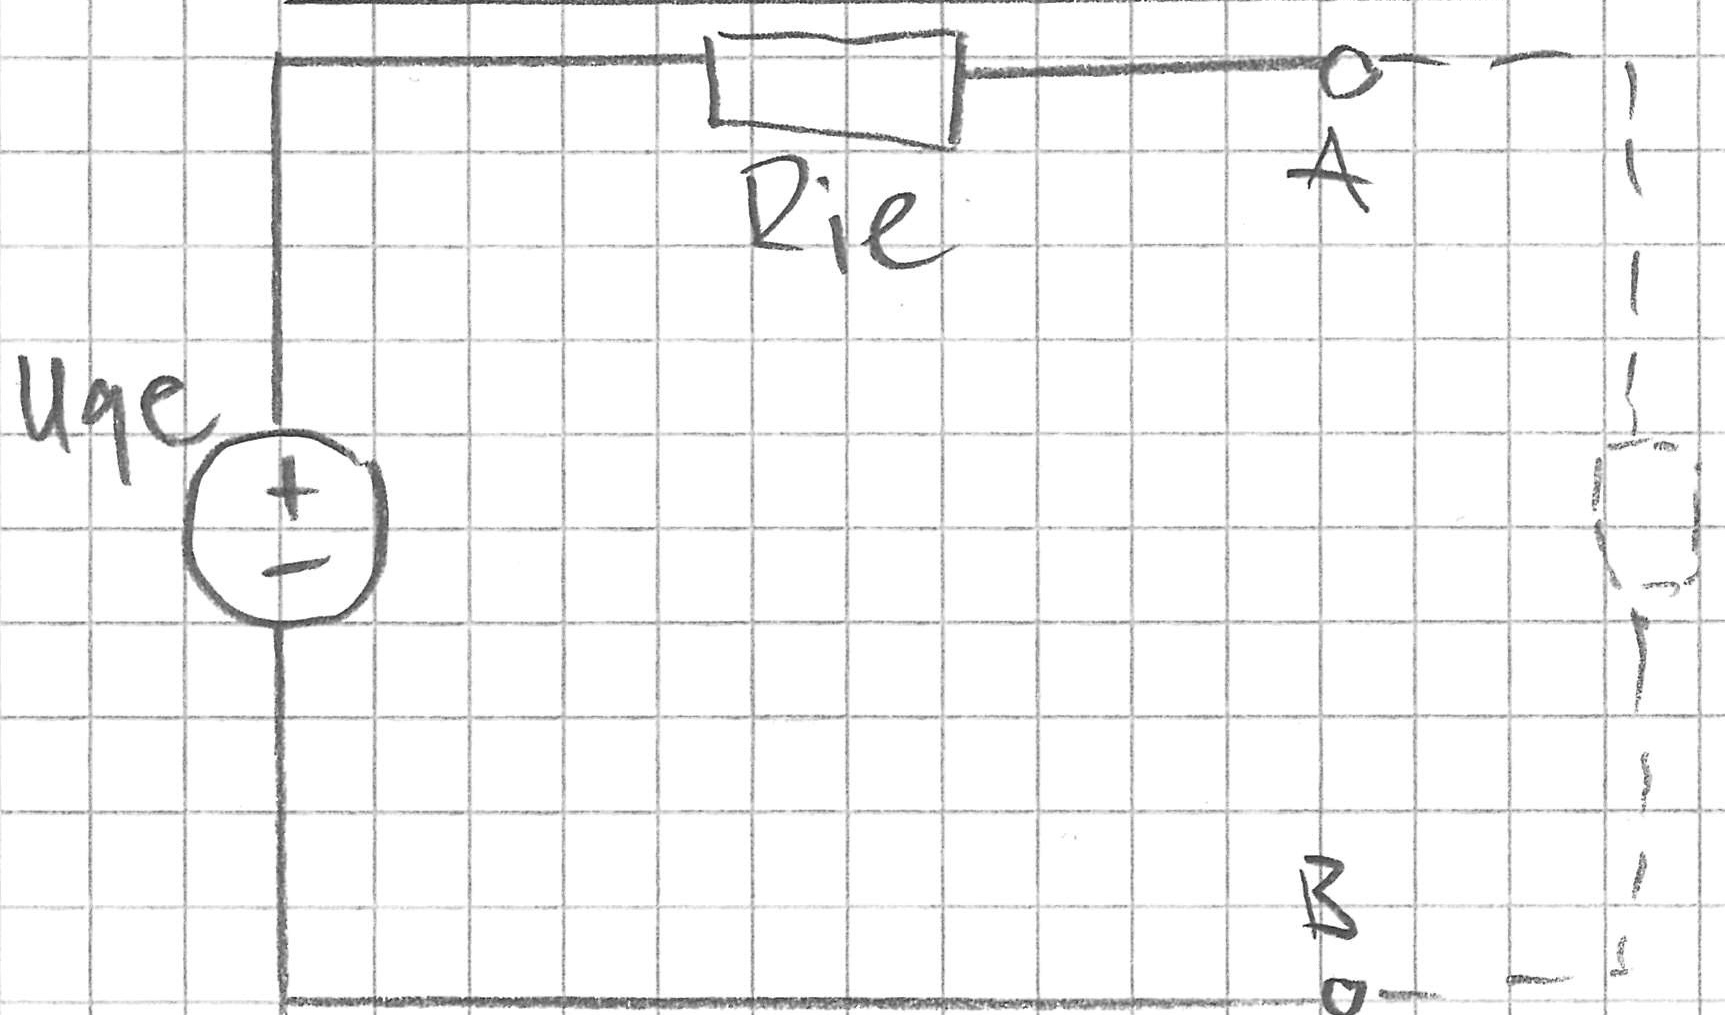
\includegraphics[width=0.25\textwidth]{pics/wheatstone/belastet} \\
$U_{AB} = Brueckenspannung$ & A-B offen: & $U_{R_L} = U_{qe} \cdot \frac{R_L}{R_{ie} + R_L}$ \\ 
abgeglichen falls $U_{AB} = 0$ & $U_{AB} = U_2 - U_4$ & $U_{qe} = U_{AB} $ von Brückenschaltung\\
d.h. $ U_2 = U_4 $ & $U_{AB} = U_0(\frac{R_2}{R_1 + R_2} - \frac{R_4}{R_3 + R_4})$ & $R_{ie} = R_1||R_2 + R_3||R_4$\\[5pt]
Abgleichbedingung: $ \frac{R_1}{R_2} = \frac{R_3}{R_4 } $ &  $ U_{BA} = U_0(\frac{R_4}{R_3+R_4} - \frac{R_2}{R_1+R_2})$& \\[-10pt]
\end{tabular}

\subsubsection{Speisung mit I-Quellen}
\begin{tabular}{lll}
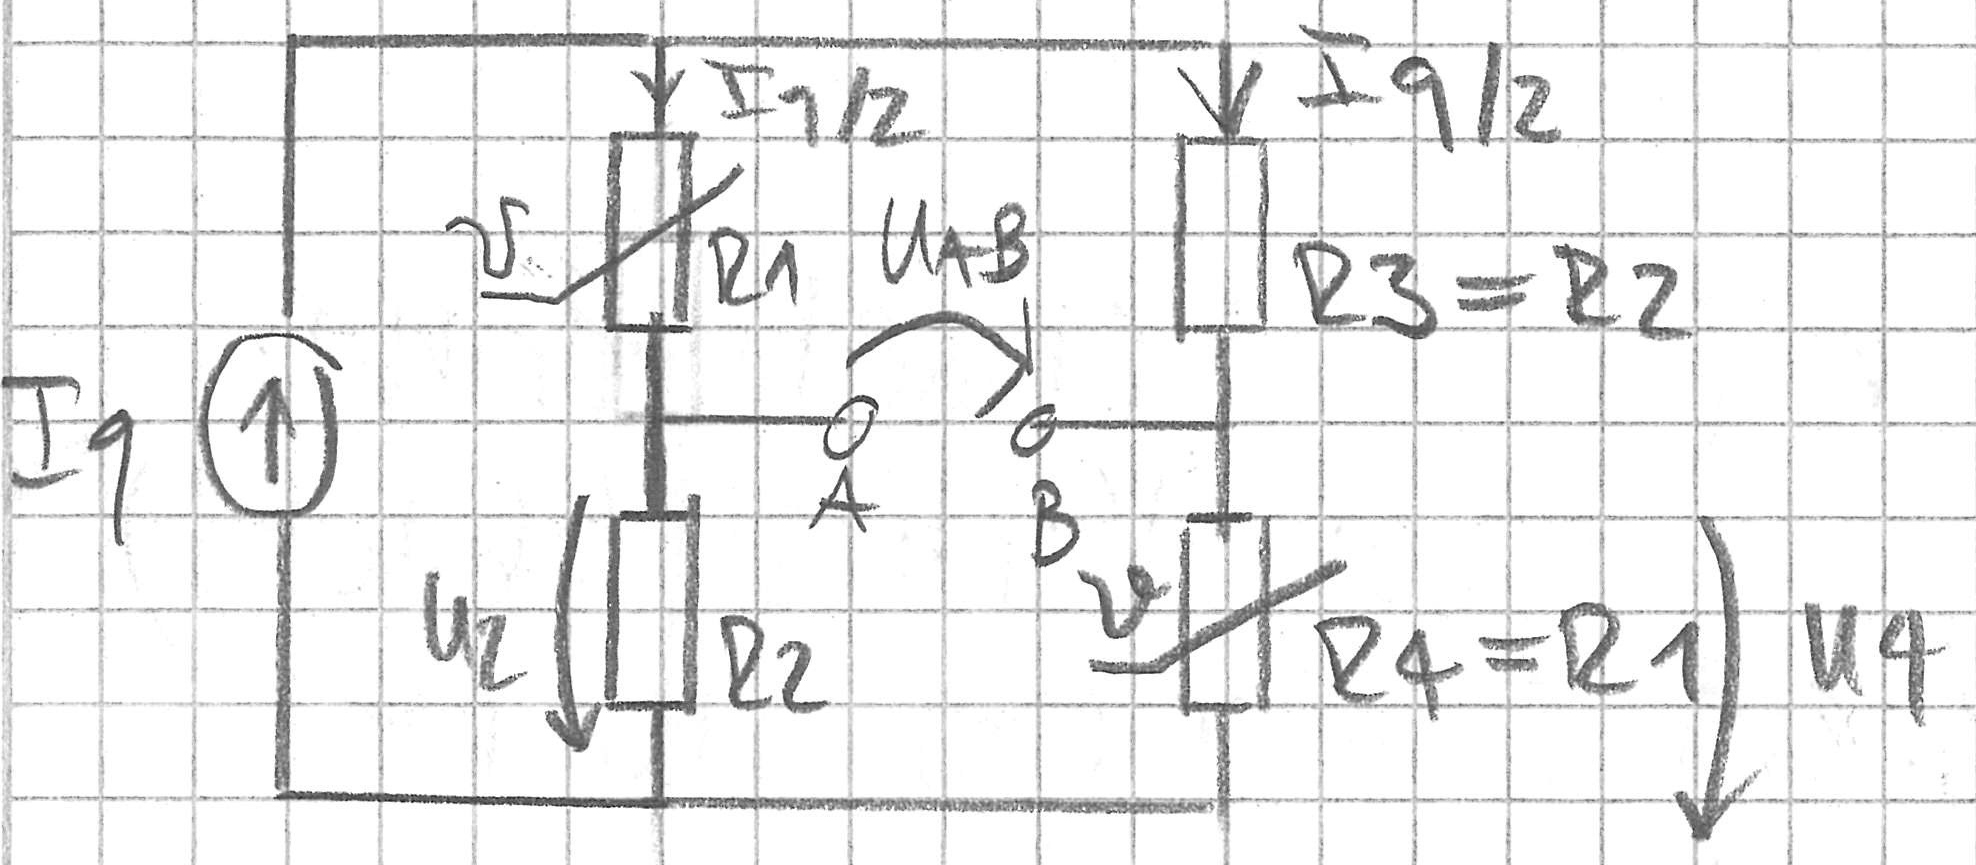
\includegraphics[width=0.3\textwidth]{pics/wheatstone/i_quelle} & 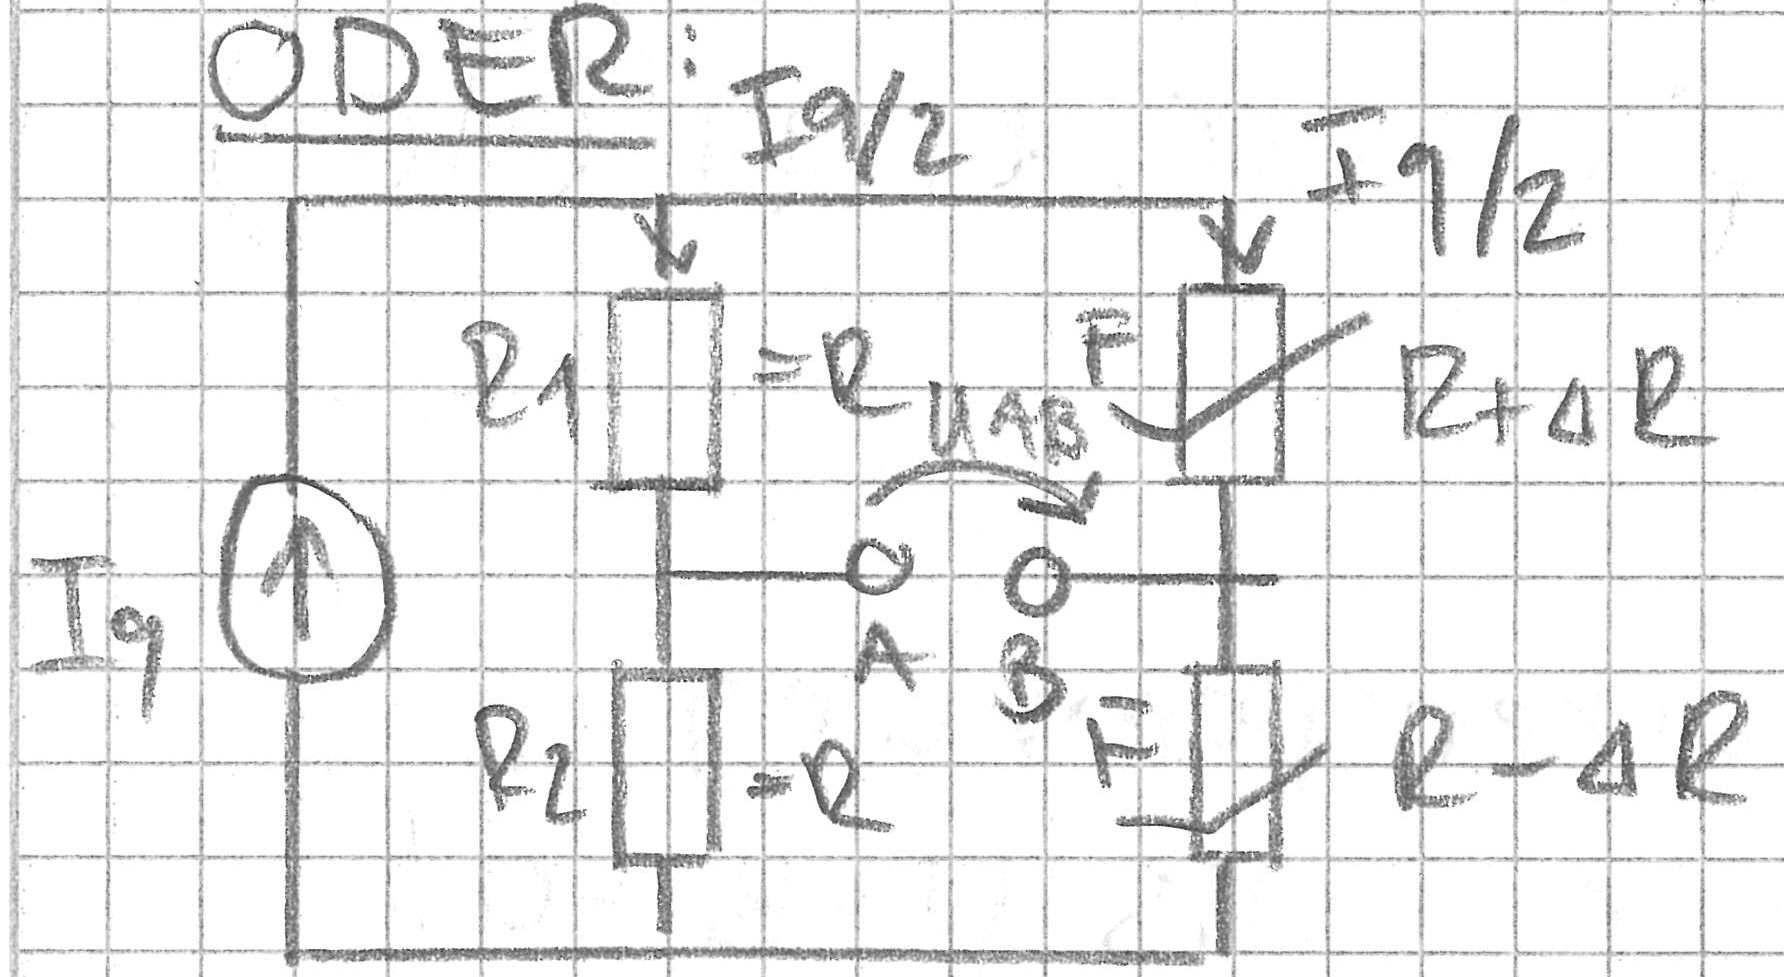
\includegraphics[width=0.25\textwidth]{pics/wheatstone/i_quelle_2}&
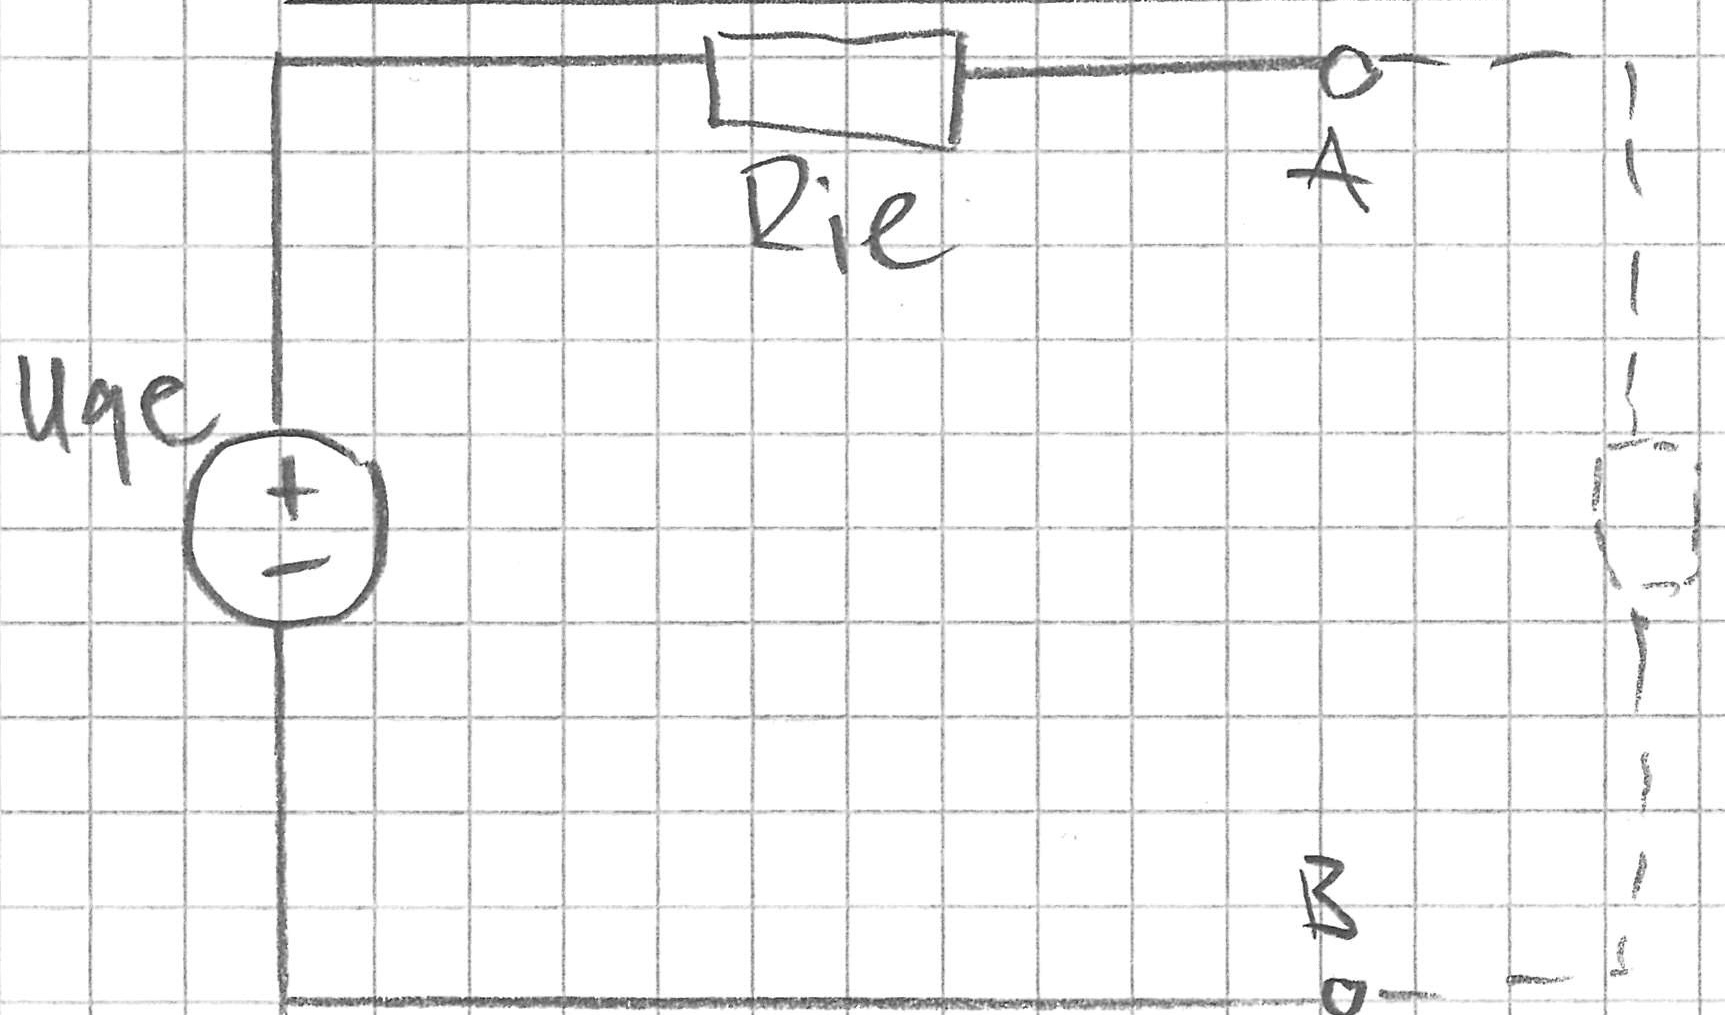
\includegraphics[width=0.25\textwidth]{pics/wheatstone/belastet} \\
$U_{AB} = U_2 - U_4$ & Ströme sind wieder gleich gross!&$U_{R_L} = U_{qe} \cdot \frac{R_L}{R_{ie} + R_L}$\\
$U_{AB} = R_2 \cdot \frac{I_q}{2} - R_4 \cdot \frac{I_q}{2}$ & $U_{AB} = \frac{I_q}{2} \cdot R - \frac{I_q}{2} \cdot (R- \Delta R)$&$U_{qe} = U_{AB} $ von Brückenschaltung\\
$\Leftrightarrow U_{AB} = \frac{I_q}{2} \cdot (R_2 - R_4)$ & $\Leftrightarrow U_{AB} = \frac{I_q}{2} \cdot \Delta R $&$R_{ie} = (R_1+R_3)||(R_2+R_4)$\\[-10pt]

\end{tabular}
